%**************************************************************************************
% License:
% CC BY-NC-SA 4.0 (http://creativecommons.org/licenses/by-nc-sa/4.0/)
%**************************************************************************************

\documentclass[notes]{beamer}

\mode<presentation> {

\usetheme{Madrid}

% Burnt orange
\definecolor{burntorange}{rgb}{0.8, 0.33, 0.0}
\colorlet{beamer@blendedblue}{burntorange}
% Pale yellow
\definecolor{paleyellow}{rgb}{1.0, 1.0, 0.953}
\setbeamercolor{background canvas}{bg=paleyellow}
% Secondary and tertiary palett
\setbeamercolor*{palette secondary}{use=structure,fg=white,bg=burntorange!80!black}
\setbeamercolor*{palette tertiary}{use=structure,fg=white,bg=burntorange!60!black}

% To remove the footer line in all slides uncomment this line
%\setbeamertemplate{footline}
% To replace the footer line in all slides with a simple slide count uncomment this line
%\setbeamertemplate{footline}[page number]

% To remove the navigation symbols from the bottom of all slides uncomment this line
%\setbeamertemplate{navigation symbols}{}
}

\usepackage{amsmath}
\usepackage{bm}
\usepackage{breqn}
\usepackage{cancel}
\usepackage{graphicx} % for figures
\usepackage{subcaption} % for subplots 
\usepackage[labelsep=space,tableposition=top]{caption}
\renewcommand{\figurename}{Fig.} 
\usepackage{cleveref}
\usepackage{caption,subcaption}% http://ctan.org/pkg/{caption,subcaption}
\usepackage{booktabs} % Allows the use of \toprule, \midrule and \bottomrule in tables
\usepackage{multirow}
\usepackage{tabularx}
\usepackage{siunitx}
\usepackage{cleveref}
\usepackage{xcolor}
\usepackage{empheq}
\usepackage[most]{tcolorbox}

\newtcbox{\mymath}[1][]{%
	nobeforeafter, math upper, tcbox raise base,
	enhanced, colframe=blue!30!black,
	colback=blue!30, boxrule=1pt,
	#1}

% To print 2 slides on a page
%\usepackage{handoutWithNotes}
%\pgfpagesuselayout{2 on 1}[border shrink=2mm]
%----------------------------------------------------------------------------------------
%	TITLE PAGE
%----------------------------------------------------------------------------------------
% The short title appears at the bottom of every slide, the full title is only on the title page
\title[CE394M: Tresca \& MC]{CE394M: Tresca and Mohr-Coulomb} 
\author{Krishna Kumar} % name
\institute[UT Austin] % institution 
{
University of Texas at Austin \\
\medskip
\textit{
  \url{krishnak@utexas.edu}} % Your email address
}
\date{\today} % Date, can be changed to a custom date

\begin{document}

\begin{frame}
\titlepage % title page as the first slide
\end{frame}

\begin{frame}
 % Table of contents slide, comment this block out to remove it
 \frametitle{Overview}
  %Throughout your presentation, if you choose to use \section{} and \subsection{} 
  %commands, these %will automatically be printed on this slide as an overview 
 \tableofcontents
\end{frame}

%----------------------------------------------------------------------------------------
% slides
%----------------------------------------------------------------------------------------
\section{Constitutive modeling}
%----------------------------------------------------------------------------------------
\begin{frame}
\frametitle{Stress invariants}
\begin{itemize}
	\item The magnitudes of the component of the stress vector depend on the chosen direction of the coordinate axes (in 3D: 6 variables).
	\item Principal stresses always act on the same planes and have the same magnitude (invariant to the coordinate axes), but still need to define the corresponding orientations (in 3D: 6 variables).
	\item For isotropic materials, it is very convenient to work with alternative invariant quantities which are combinations of principal stresses.
\end{itemize}
\end{frame}

%----------------------------------------------------------------------------------------
\begin{frame}
\frametitle{Stress invariants}
\begin{itemize}
	\item Mean effective stress $p = \frac{1}{3}(\sigma_I + \sigma_II + \sigma_III)$
	\item Deviatoric stress: $J = \frac{1}{\sqrt{6}}\sqrt{(\sigma_I - \sigma_{II})^2 + (\sigma_{II} - \sigma_{III})^2 + (\sigma_{III} - \sigma_I)^2}$
	\item Lode's angle $\theta = \tan^{-1}\left[\frac{1}{\sqrt{3}}\left(2\frac{(\sigma_{II} - \sigma_{III})}{\sigma_I - \sigma_{III}} -1 \right)\right]$
\end{itemize}

Principal stresses can be expressed in terms of invariants:

\begin{equation*}
\begin{bmatrix}
\sigma_I \\
\sigma_{II} \\
\sigma_{III} \\
\end{bmatrix} = 
p \begin{bmatrix}
1 \\
1 \\
1 \\
\end{bmatrix} + 
\frac{2}{\sqrt{3}}J
\begin{bmatrix}
\sin\left(\theta + \frac{2 \pi}{3}\right) \\
\sin \theta \\
\sin\left(\theta - \frac{2 \pi}{3}\right) \\
\end{bmatrix}
\end{equation*}
\end{frame}

\section{Tresca model}
%----------------------------------------------------------------------------------------
\begin{frame}
\frametitle{Tresca model}
Simulation of undrained behavior of saturated clay

Failure criteria: 
\mode<beamer>{
	\begin{equation*}
		\tau_f = s_u
	\end{equation*}
where $\tau_f$ is the shear stress at failure. $s_u$ is the undrained strength.
}
\mode<handout>{
	\vspace{1.5cm}
}
\begin{figure}
	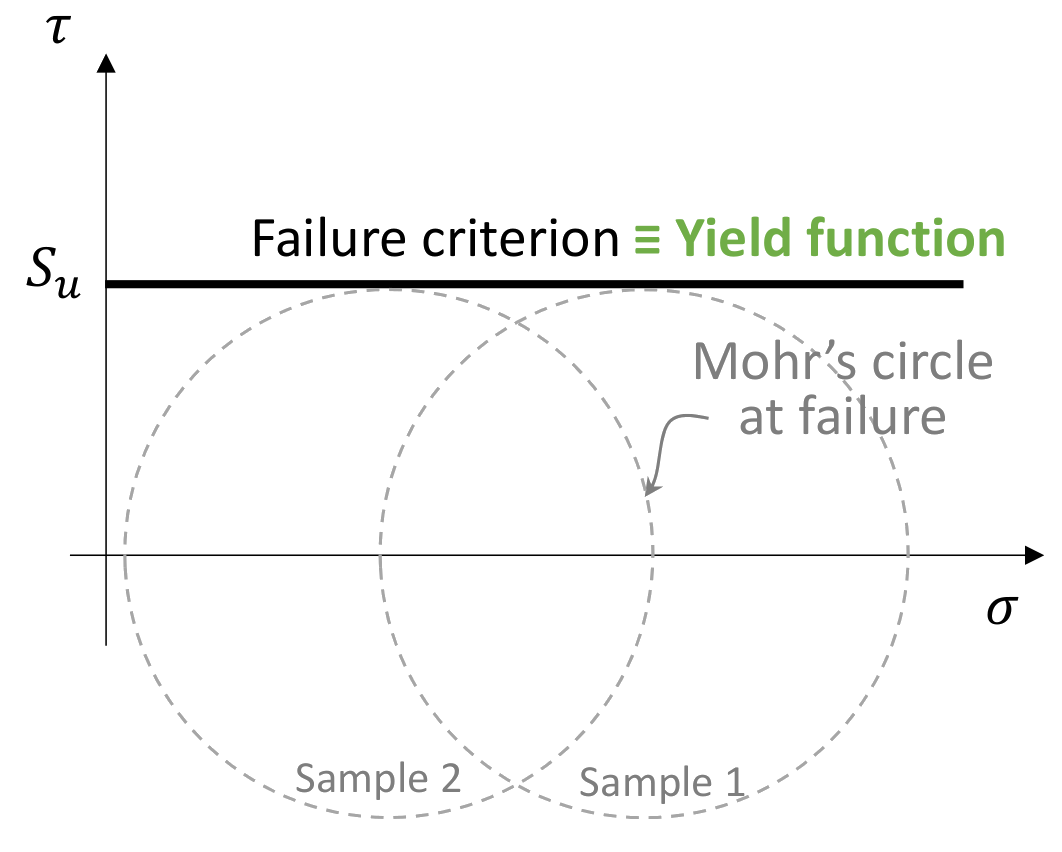
\includegraphics[width=0.55\textwidth]{figs/tresca.png}
\end{figure}
\end{frame}

%----------------------------------------------------------------------------------------
\begin{frame}
\frametitle{Tresca model}
Yield function
\mode<beamer>{
	\begin{align*}
	F (\sigma, W_p) & = \sigma_I - \sigma_{III} - 2 s_u = 0 \\
	& = J \cos \theta - s_u = 0 
	\end{align*}
}
\mode<handout>{
	\vspace{1.5cm}
}
\begin{figure}
	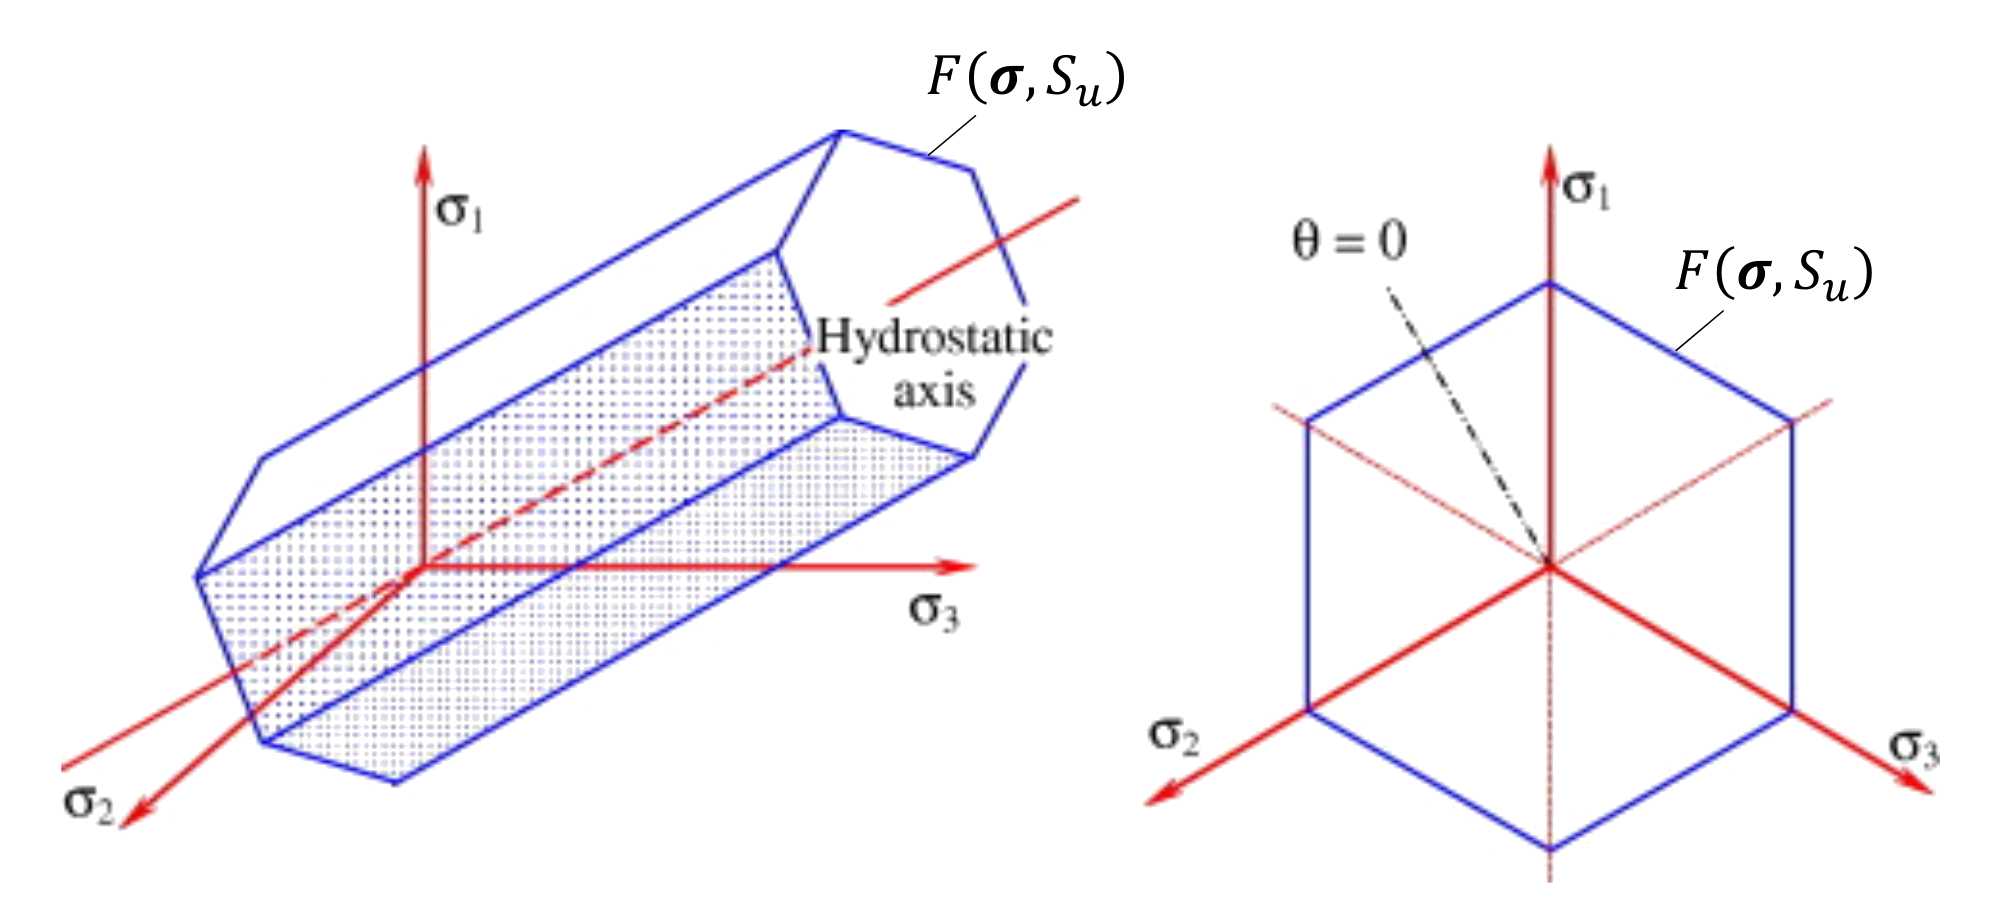
\includegraphics[width=\textwidth]{figs/tresca-yield.png}
\end{figure}
\end{frame}

%----------------------------------------------------------------------------------------
\begin{frame}
\frametitle{Tresca model}

\mode<beamer>{
	\begin{enumerate}
		\item The model is intended to predict the undrained behavior of
		saturated clay, hence it should predict zero volumetric strains.
		\item This fact constrains the plastic potential, and an associated flow rule should be considered.
		\item In general, this is a perfectly plastic model (no hard/soft law)
		\item Parameters required (3): $s_u, E_u, \nu_u$.
	\end{enumerate}
}
\mode<handout>{
	\vspace{2cm}
}
\begin{figure}
	\includegraphics[width=0.8\textwidth]{figs/tresca-su.png}
\end{figure}
\end{frame}

\section{Mohr-Coulomb model}

%----------------------------------------------------------------------------------------
\begin{frame}
\frametitle{Mohr-Coulomb model}

\mode<beamer>{
	Failure criteria: $\tau_f = c^\prime = \sigma^\prime_f \tan \phi^\prime.$
	
	\begin{equation*}
	F(\sigma^\prime, c^\prime, \phi^\prime) = \frac{1}{2}(\sigma_I^\prime - \sigma_{III}^\prime) - \frac{1}{2}(\sigma_I^\prime + \sigma_{III}^\prime) \sin \phi^\prime - c^\prime \cos \phi^\prime = 0.
	\end{equation*}
}
\mode<handout>{
	\vspace{2cm}
}
\begin{figure}
	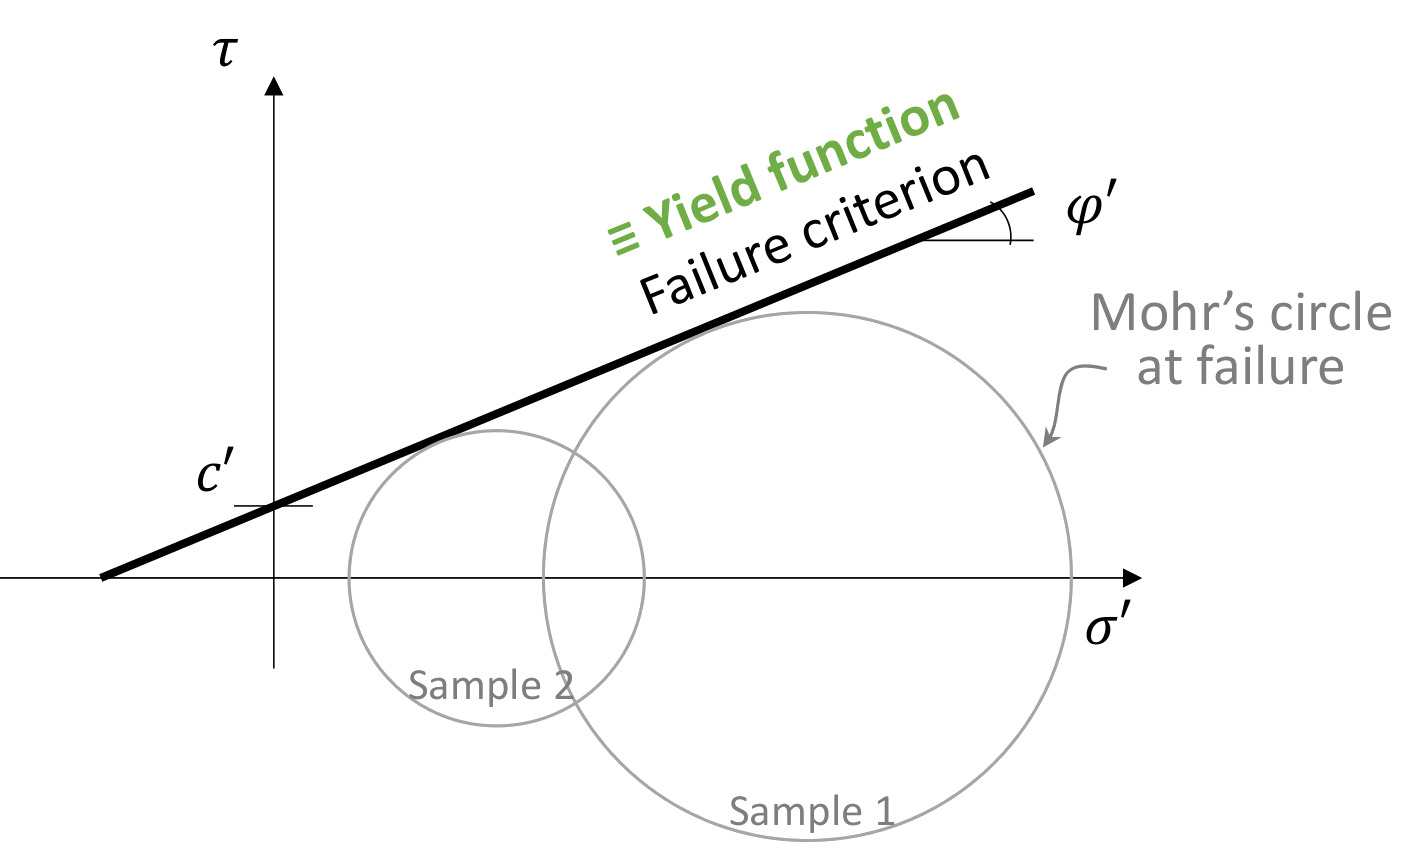
\includegraphics[width=0.8\textwidth]{figs/mohr-coulomb.png}
\end{figure}
\end{frame}

%----------------------------------------------------------------------------------------
\begin{frame}
\frametitle{Mohr-Coulomb model}
\begin{figure}
	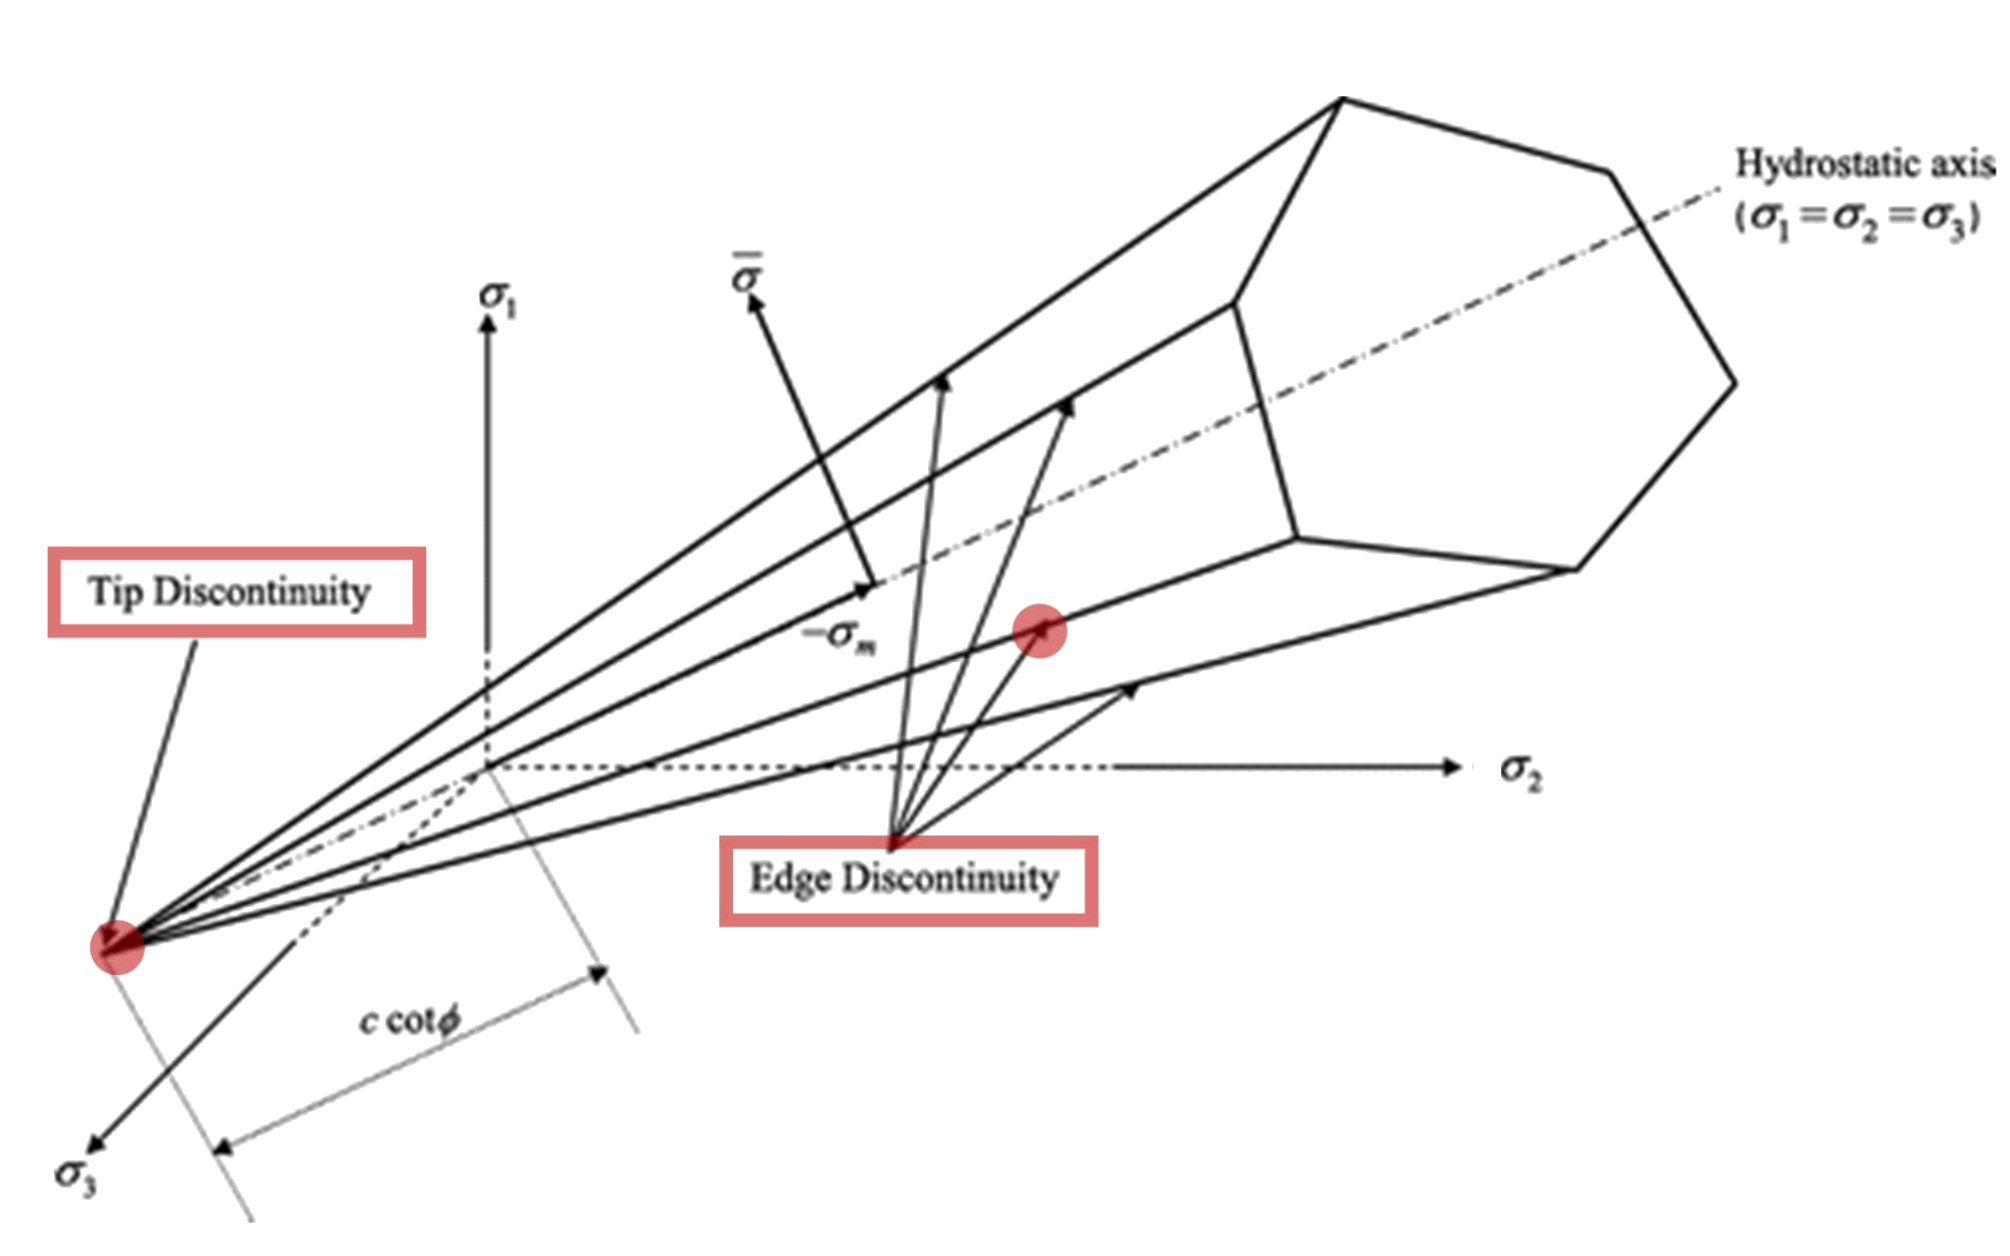
\includegraphics[width=\textwidth]{figs/mc-yield.png}
\end{figure}
\end{frame}

%----------------------------------------------------------------------------------------
\begin{frame}
\frametitle{Mohr-Coulomb: flow rule?}
Can we consider an associative flow rule?
\mode<beamer>{
	Failure criteria: $	F(\sigma^\prime, c^\prime, \phi^\prime) = 	G(\sigma^\prime, c^\prime, \phi^\prime)$
}
\mode<handout>{
	\vspace{1cm}
}
\begin{figure}
	\includegraphics[width=0.6\textwidth]{figs/mc-flow.png}
\end{figure}
\mode<beamer>{
$\varepsilon^p$ is inclined at an angle of $\phi^\prime$, and indicates negative (tensile) plastic strains. This results in a dilatant volumetric plastic strain $(d\varepsilon^p_{vol})$, in which the angle of dilation $\psi$ is equal to the effective friction angle $(\phi^\prime)$.
}
\mode<handout>{
	\vspace{1.5cm}
}
\end{frame}

%----------------------------------------------------------------------------------------
\begin{frame}
\frametitle{Mohr-Coulomb: Drawbacks (associative)}
\mode<beamer>{
	\begin{enumerate}
		\item The magnitude of the plastic volumetric strains $(d\varepsilon)$ is much larger than that observed in real soils.
		\item Once the soil yields it will dilate for ever! (note: real soil, which may dilate initially on meeting the failure surface,
		will often reach a constant volume condition at large strains).
	\end{enumerate}
}
\mode<handout>{
	\vspace{2.5cm}
}
\textbf{Solutions:}
\mode<beamer>{
	\begin{enumerate}
		\item Adopt a non‐associated flow rule with a more realistic angle of dilation $\psi$
		\item Allow angle of dilation vary with plastic strain (hardening/softening law) $\psi = f(\varepsilon)$
	\end{enumerate}
}
\mode<handout>{
	\vspace{2.5cm}
}
\end{frame}

%----------------------------------------------------------------------------------------
\begin{frame}
\frametitle{Mohr-Coulomb: non-associative model}
\mode<beamer>{
	Consider a non-associated model with $\psi = 0$. In which case $d\varepsilon_{vol}^p = 0$.
	
	Parameters (5): $c^\prime, \phi^\prime, \psi, E, \nu$.
}
\mode<handout>{
	\vspace{2cm}
}
\begin{figure}
	\includegraphics[width=0.8\textwidth]{figs/mc-non-associated.png}
\end{figure}
\end{frame}

%----------------------------------------------------------------------------------------
\begin{frame}
\frametitle{Mohr-Coulomb: Yield and Potential fn}
\mode<beamer>{
	Yield fn: $F = \sigma_1^\prime - \sigma_3^\prime N_\phi + 2 c \sqrt{N_\phi} = 0$., where $N_\phi = \frac{1 + \sin\phi^\prime}{1 - \sin\phi^\prime}$
	
	Potential fn: $G = \sigma_1^\prime - \sigma_3^\prime N_\psi + constant = 0$., where $N_\psi = \frac{1 + \sin\psi^\prime}{1 - \sin\psi^\prime}$ 
}
\mode<handout>{
	\vspace{1cm}
}
\begin{figure}
	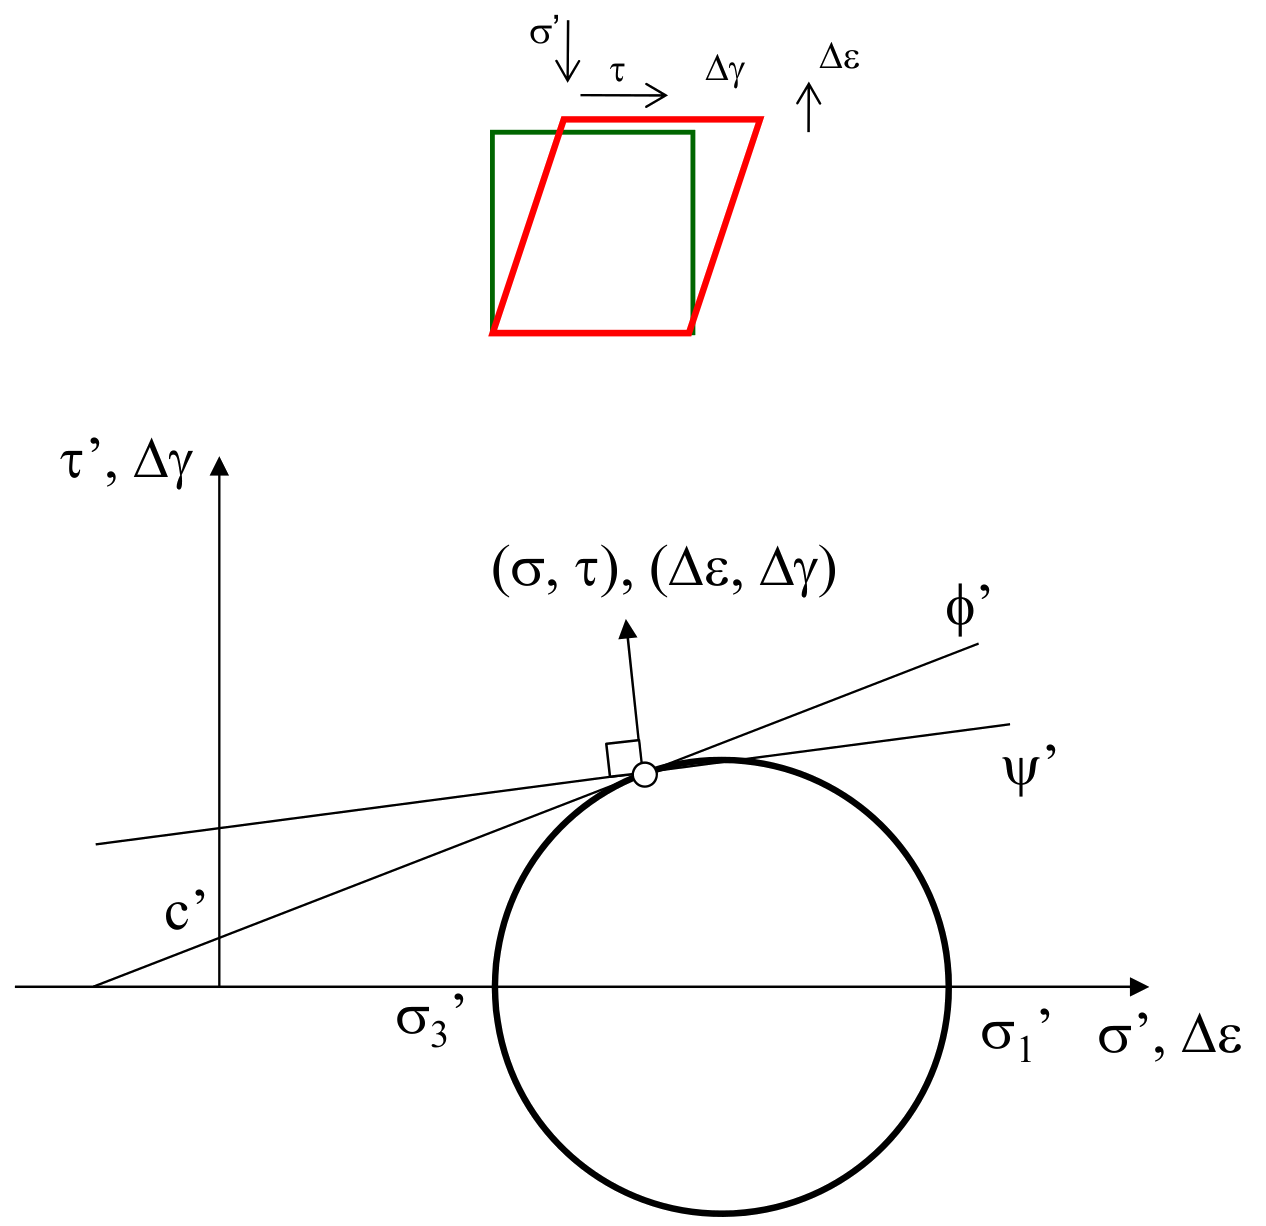
\includegraphics[width=0.5\textwidth]{figs/mc-yield-potential.png}
\end{figure}
\end{frame}


%----------------------------------------------------------------------------------------
\begin{frame}
\frametitle{Mohr-Coulomb: plastic strains}
\mode<beamer>{
	\begin{align*}
	d\varepsilon_1^p & = \lambda \frac{\partial G}{\partial \sigma_1} = \lambda \cdot 1 = \lambda \\
	d\varepsilon_2^p & = \lambda \frac{\partial G}{\partial \sigma_2} = \lambda \cdot 0 = 0 \quad \text{Zero strain increment in 2-dir}\\	
	d\varepsilon_3^p & = \lambda \frac{\partial G}{\partial \sigma_3} = \lambda \cdot (-N_\psi) = -\lambda N_\psi\\	\end{align*}
}
\mode<handout>{
	\vspace{2.5cm}
}
\begin{figure}
	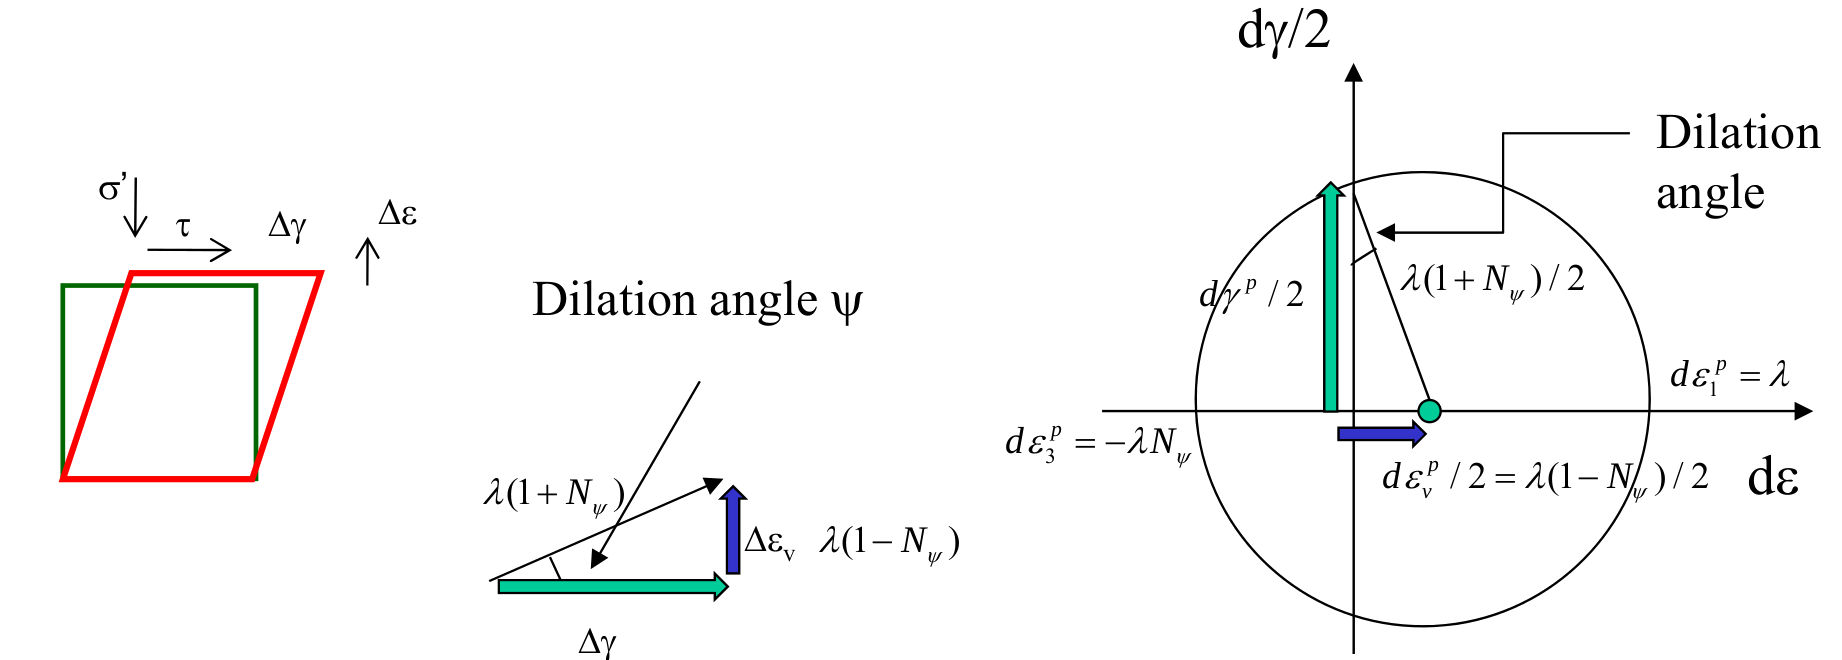
\includegraphics[width=0.8\textwidth]{figs/plastic-strains.png}
\end{figure}
\end{frame}



%----------------------------------------------------------------------------------------
\begin{frame}
\frametitle{Interpretation of drained TXC}
	
\noindent
\fboxsep=0pt
\noindent
\begin{minipage}[t]{0.48\linewidth}
Plastic volumetric strain:
\mode<beamer>{
	\begin{align*}
	d\varepsilon_v^p & = d \varepsilon_1^p + d \varepsilon_2^p + d \varepsilon_3^p = \lambda (1 - N_\psi) \\
	& = \lambda \frac{2 \sin \psi}{1 - \sin \psi} \\
	\frac{d\varepsilon_v^p}{d\varepsilon_1^p} & = \frac{\frac{2 \sin \psi}{1 - \sin \psi}}{\lambda} = \frac{2 \sin \psi}{1 - \sin \psi}
	\end{align*}
}
\mode<handout>{
	\vspace{2.5cm}
}
\end{minipage}%
\hfill%
\begin{minipage}[t]{0.48\linewidth}
	Note that $\psi$ changes with plastic
	strain in real soils
	\begin{figure}
		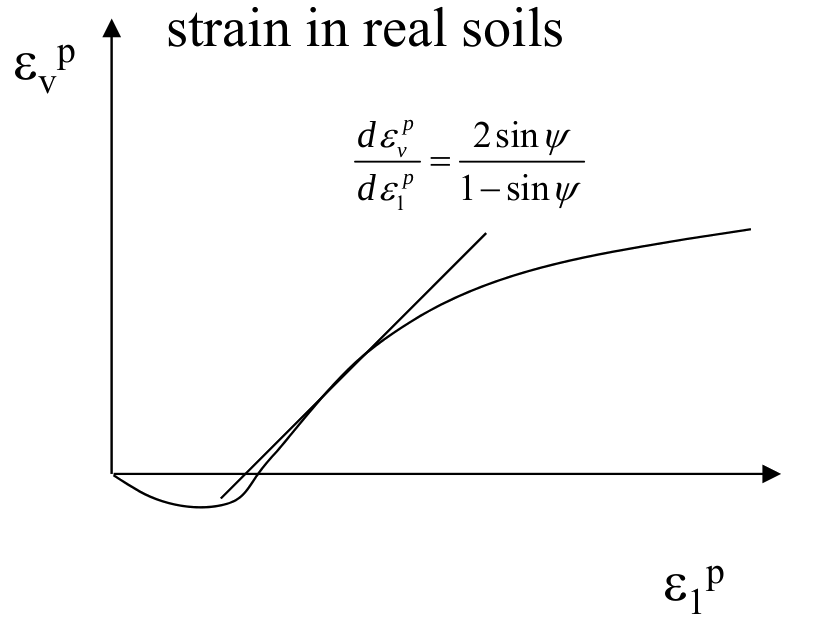
\includegraphics[width=0.6\textwidth]{figs/mc-drained-txc.png}
	\end{figure}
\end{minipage}
\begin{figure}
	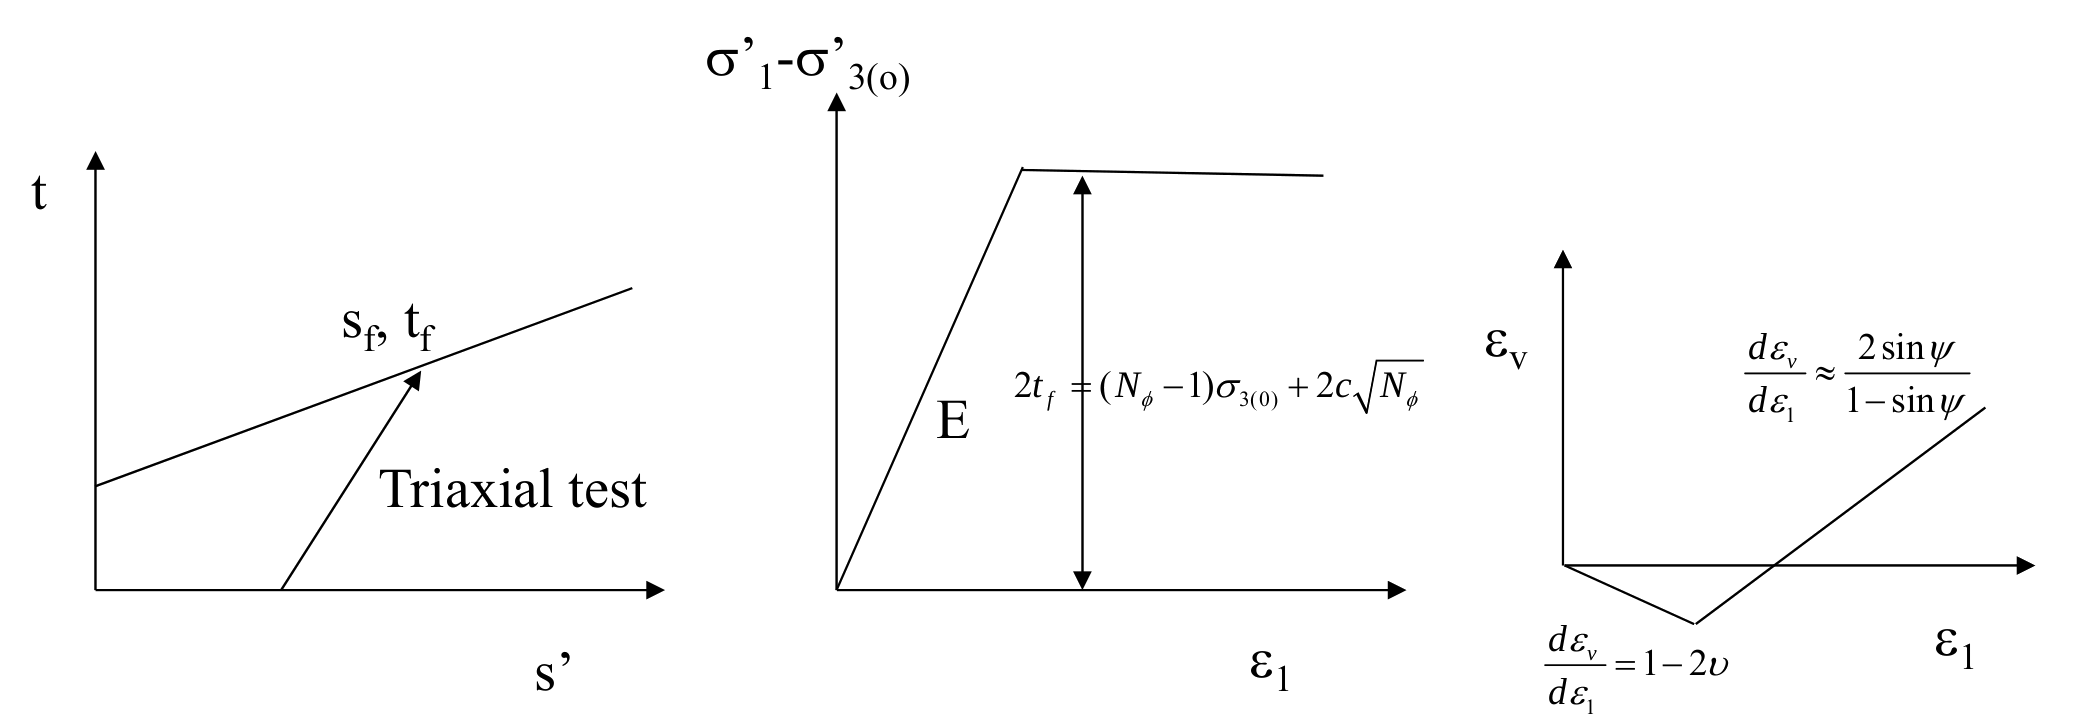
\includegraphics[width=0.9\textwidth]{figs/idealized-mc.png}
	\caption*{Idealized M-C curves}
\end{figure}
\end{frame}

%----------------------------------------------------------------------------------------
\begin{frame}
\frametitle{Mohr-Coulomb: Tension cut-off}
\mode<beamer>{
	\begin{enumerate}
		\item For $c=0$, the standard Mohr‐Coulomb criterion allows for tension.
		Allowable stress increase with cohesion.
		\item In reality, soil can sustain none or only very small tensile stresses.
		\item This behavior is usually included by specifying a tension cut‐off, which is equivalent to include an additional yield surface: $F(\sigma, \sigma_t) = \sigma_i - \sigma_t = 0$.
	\end{enumerate}
}
\mode<handout>{
	\vspace{3cm}
}
\begin{figure}
	\includegraphics[width=0.6\textwidth]{figs/mc-non-associated.png}
\end{figure}
\end{frame}
\end{document}
